% !TEX root = ../main.tex

\chapter{Literature Review}\label{ch:literature}
In this chapter we will look at previous works in areas relevant to this report.
This chapter looks at how these pieces of work have developed and the methods of studying them with computer models. 

\section{Background}\label{sec:background}
The PD and its a large area of repeated games in GT and has applications in the real world.
This is due to the game being a good example of strategies that give a cooperative benefit to repeated games.
The PD was first formally presented by Albert W. Tucker~\cite{cambell2016thesis, gass2005annotated} and the iterated version was made famous by Robert Axelrods work in the 1980s~\cite{axelrod1980effective}.
It has been used to describe actions of people and governments in situations stretching from warfare~\cite{tooby1988war,aumann1992handbook}and finance~\cite{cable1997finance} to politics~\cite{snidal1985Politics} and sexual relationships~\cite{low2015sex}.
Because of its applicability to real world scenarios there is a strong desire to understand how strategies are beaten to either exploit flaws or counter opponents in real world scenarios.

The Prisoners dilemma became a large research area in the combination of mathematics and computer science after Robert Axelrod published his work named `Effective Choice In The Prisoners Dilemma'~\cite{axelrod1980effective}.
In it he makes an introduction to how tournaments are run and the properties of successful results.
His method of experimenting became the standard for handling the IDP problem.
This was the first example of computer tournaments, for which he had to as for code programs which had inputs of the history for both players and resulted in an output move for that next turn.
After the tournament is complete he describes what successful strategies had in common; 
It turns out the majority of successful strategies, including the winner, Tit For Tat, have properties of niceness and forgiveness.
Niceness is the property of not defecting to start and forgiveness is the property of forgetting previous defections in a timely manner.
This allowed them to thrive in the tournament and have overall scores that rose above strategies without niceness or forgiveness.

Since Axelrods' original tournament there have been many research papers on what makes a successful strategy for a specific objective.
For example William H Press and Freeman J Dyson,~\cite{press2012iterated}, looked at how to it is possible to deterministically set an opponents score and Shashi Mittal and Kalyanmoy Deb have looked at a range of different objectives at once~\cite{mittal2009optimal}.
These specific objectives are the core part of applying Game Theory and the Prisoners Dilemma in the real word~\cite{rehmeyer2012climateNegotiations,osang2013environmental,Schneier2012doping}.
Objectives are the wrapper for which we can work with real world scenarios, for example in a the cold war it was not the goal to get as many missiles as possible to pass an oppositions defence but to not allow any missiles through your own defence; i.e.minimising your opponents score.
In a football tournament where winning is the number or goals your team scores it does not matter how many goals you get in so long as you score the most overall.
This leads to observing that the IPD describes that a players world is better if their opponent is cooperative.  
There are also some very useful applications such as rent splitting or work assignments~\cite{goldman2015spliddit}, all of which were programmed and deployed to a website for general use online~\cite{spliddit}.

\section{Strategy Structures}\label{sec:stratergyStructures}
A strategy is a way of defining how to play the IPD. 
It is a way of identifying which move to play next based on some parameters; for example the strategy of all $C$ moves is valid, as is a wildly complicated description of what to do based on the last 20 moves of an opponent.

Individual strategies can be defined in multiple ways~\cite{harper2017reinforcement}.
Each method of representing a strategies has its benefits and drawbacks, typically due to fundamental properties of the strategy (like being stochastic) or that it is more concise to write in a certain method.
There are methods of creating strategies that remove the way opponents play in order to create overall scores that desired.
Ways of structuring a strategy are shown below:

\begin{itemize}
 \item LookerUpper, for example figure~\ref{fig:tit_for_tat_LUD}.
 \item Gambler, for example the Stochastic stratergies; examples can be found in~\cite{press2012iterated}.
 \item Neural Networks.
 \item Finite State Machines, for example figure~\ref{fig:tit_for_tat_FSD}.
 \item Hidden Markov Models.
 \item Explicit Move List, for example the solutions given in Appendix~\ref{apndx:solutionGroups}.
 \item Mixtures.
\end{itemize}

\subsection{Equivalent Strategies}\label{subsec:equivalentStrategies}
Looking at certain opponents there are occasions some strategies that look indistinguishable from others;
for example two stochastic opponents can can be incredibly similar, but identifying which one is which from their play history could be impossible.
One of the ways we are able to identify strategies is the process of fingerprinting~\cite{Ashlock2004,Ashlock2008,cambell2016thesis}.
However this can be inconclusive and less accurate as desired.
An effective method of identifying equivalent strategies is to write them down in the form of the other.
For example if we can write any strategy in one of the forms given in figures~\ref{fig:tit_for_tat_FSD},\ref{fig:tit_for_tat_LUD} we know its an equivalent to Tit for Tat.

The work being completed in this paper is another method of identifying strategies; identifying the best response to them may lead to observations about how and why different strategies act in similar manners.
This wont lead to show strategy equivalence, but it will show how solution equivalence.

\begin{figure}[ht]
    \centering
    \begin{minipage}{0.48\textwidth}
        \centering
        \tikzset{EdgeStyle/.append style = {->} ,
        LabelStyle/.style = {rectangle, rounded corners, draw, fill = black!5}}
        \begin{tikzpicture}[
            startnode/.style={rectangle, rounded corners, draw, fill = blue!5},
            roundnode/.style={circle, draw=black!60, fill=green!10, very thick, minimum size=7mm}
            ]
            %Nodes
            \node[roundnode](initial_state){1}; 
            \node[startnode](start_node)[left=of initial_state]{Start};
            %Lines
            \Edge[label = $C$](start_node)(initial_state)
            \Loop[dist = 3cm, dir = NO, label = $C/C$](initial_state.north)
            \Loop[dist = 3cm, dir = SO, label = $D/D$](initial_state.south)
        \end{tikzpicture}
        \caption{Finite State diagram of strategy Tit for Tat}\label{fig:tit_for_tat_FSD}
    \end{minipage}\hfill
    \begin{minipage}{0.48\textwidth}
        \centering
        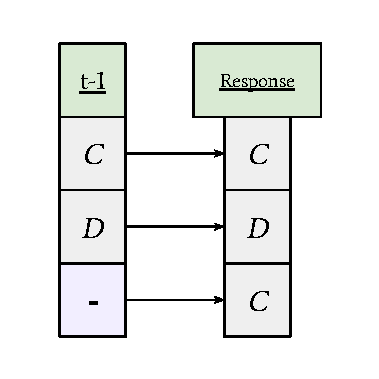
\includegraphics[width=0.6\textwidth, center]{./img/examples/tit_for_tat_LUD.pdf}
        \caption{Look Up diagram of strategy Tit for Tat}\label{fig:tit_for_tat_LUD}
    \end{minipage}
\end{figure}


\section{Strategies Of Interest}\label{sec:strategiesOfInterest}
\textbf{Tit For Tat} was the winner of the original axelrod tournament in 1980~\cite{axelrod1980effective}. It s a very basic opponent who has strong forgiveness (it will forgive a defection after 1 move) and generosity (it will start with a cooperation) which is thought to give its well overall score in tournaments.

\textbf{Alternator} is a `dumb' opponent, i.e. no strategic method at all. All it will do is alternate between cooperation and defection until the game ends. 
Playing against an Alternator effectively is to defect the whole game; identifying an alternator to play this sequence of defections without backlash can be difficult.
If we are playing a similar starting strategy such as Collective Strategy defecting in the first two moves will cause us to sore badly overall.

\textbf{Grudger} can be considered as the most unforgiving strategy that exists.
Starting by cooperating, if you defect even once then the Grudger will defect until the end of the game.
In line with Tit For Tat, our best score will come from not `upsetting' the opponent (until the last move where it cant react.

\textbf{Random} is the most basic stochastic opponent, and like Alternator and Cycler it is `dumb'. 
With a probability $p$ of cooperating and $1-p$ of defecting, we can just defect the whole time to beat this opponent; picking up bonus points on its cooperation moves.

\textbf{EvolvedFSM16} is a 16 state Finite State Machine (FSM) that has been trained with an evolutionary algorithm. It has been optimised for tournament matches, the definition can be found in the axelrod documentation~\cite{axelrodproject}.

\textbf{CollectiveStrategy} was defined in~\cite{li2009strategy}. ‘It always cooperates in the first move and defects in the second move. If the opponent also cooperates in the first move and defects in the second move, CS will cooperate until the opponent defects. Otherwise, CS will always defect.’

\textbf{ZDExtortion} is first mentioned in the paper \textit{Iterated Prisoner’s Dilemma contains strategies that dominate any evolutionary opponent}~\cite{press2012iterated}. In it the authors discuss methods of extorting score from another player. We use this player an example of a difficult to beat player.

\textbf{Cycler} is a strategy which cycles and repeats a sequence until the end of the match. 
For example \mintinline{python}{cycler("CCD")} will play C$2,1,2,1,2,\ldots$ for as long as necessary.
The Cycler strategy will be directly used in the GA by using the current solution, of length 200, as the parameter to play a specific absolute sequence during a generations scoring round.
This cycler class will contain our solution sequence and the sequence can be extracted for mutation \& crossover as needed.

\section{Genetic Algorithms}
This work will focus on GAs which are a specific form of ML.
Advanced techniques of machine learning can be combined and used together\footnote{Techniques for teaching and versioning static algorithms such as building a `clever' game AIs, where the core concept of the AI is fine tuned using a GA in an development environment but isn't implemented into the game~\cite{bakkes2009rapid}.} in many situations, lots of these techniques combine genetic algorithms or some sort of fitness testing within a larger scope.
The field of mathematics research is one which has plenty of examples of GAs in action;
for example the same techniques as we will using is used in~\cite{chu1997genetic} to solve the Generalised Assignment Problem.
Another example, \cite{bhanu1995adaptive}, used neural networks when approaching the state regulation problem.

\section{Conclusion}
In this chapter we have looked at previous work and how they influence the work contained in this report.
Most importantly we have looked at how strategies can be linked together through certain properties, such as their structure.
As we continue looking at solutions for certain strategies we will be constructing another grouping of strategies in their solution sequences.
This may lead to finding similarities to opponents who seem to have vastly different in structure.
